\begin{filecontents*}[overwrite]{sources_v3_2.bib}
@online{inspiration,
  author = {Instructables},
  title = {Building a Self-Driving Boat: ArduPilot Rover},
  url = {https://www.instructables.com/Building-a-Self-Driving-Boat-ArduPilot-Rover/},
  urldate = {2026-11-05}
}

@online{coreDoc,
  author = {ArduPilot},
  title = {CoreWing F405 Wing V2 / Wing Mini V2, Rover documentation},
  url = {https://docs.ardupilot.org/rover/docs/common-CoreWingF405WingV2.html},
  urldate = {2026-11-05}
}

@online{coreShop,
  author = {Shopee Malaysia: RC Official Store},
  title = {CoreWing F405 Mini V2, variant-priced seller listing},
  url = {https://shopee.com.my/COREWING-F405-Mini-V2-Fixed-Wing-Flight-Controller-STM32F405-OSD-VTOL-MicroSD-Card-Blackbox-Support-2-6S-LiPo-ArduPilot-INAV-for-FPV-RC-Airplane-i.23419821.55017808886},
  urldate = {2026-11-05}
}

@online{speedDoc,
  author = {SpeedyBee},
  title = {SpeedyBee F405 V4 BLS 60A 30x30 FC and ESC stack technical specifications},
  url = {https://www.speedybee.com/speedybee-f405-v4-bls-60a-30x30-fc-esc-stack/},
  urldate = {2026-11-05}
}

@online{speedAP,
  author = {ArduPilot},
  title = {Speedy Bee F4 V3/V4, Rover board documentation},
  url = {https://docs.ardupilot.org/rover/docs/common-speedybeef4-v3.html},
  urldate = {2026-11-05}
}

@online{speedShop,
  author = {Shopee Malaysia: kfhobby.my},
  title = {SpeedyBee F405 V4 60A BLS flight controller and ESC stack},
  url = {https://shopee.com.my/SpeedyBee-F405-V4-60A-BLS-3-6s-4-in-1-8-Bit-30x30-Flight-Controller-Stack-for-5-8-inch-Frame-Drone-FPV-Freestyle-Drone-Model-i.1929816412.27245780683},
  urldate = {2026-11-05}
}

@online{jetShop,
  author = {Shopee Malaysia: Creative8.my},
  title = {12V three-blade underwater jet motor; motor variants},
  url = {https://shopee.com.my/RC-Boat-12V-Jet-Boat-Underwater-3-blades-Propeller-Motor-Engine-Thruster-for-DIY-RC-ROV-Robot-Bait-Boat-Submarine-i.867757154.29083229097},
  urldate = {2026-11-05}
}

@online{mdd10,
  author = {Cytron},
  title = {MDD10A 10A 5-30V two-channel brushed DC motor driver},
  url = {https://my.cytron.io/c-motor-driver/c-dc-motor-driver/p-10amp-5v-30v-dc-motor-driver-2-channels},
  urldate = {2026-11-05}
}

@online{mdd3,
  author = {Cytron},
  title = {MDD3A 3A 4-16V two-channel brushed DC motor driver},
  url = {https://my.cytron.io/c-motor-driver/c-dc-motor-driver/p-3amp-4v-16v-dc-motor-driver-2-channels},
  urldate = {2026-11-05}
}

@online{hobbyShop,
  author = {Shopee Malaysia: YSIDO Store},
  title = {Hobbyocean underwater thruster 16V 300W 40A ESC variants},
  url = {https://shopee.com.my/Hobbyocean-Underwater-Thruster-Combo-Brushless-Motor-16V-300W-With-40A-ESC-for-RC-Bait-Tug-Boat-Nest-Ship-Submarin-ROV-Robot-i.487084356.44255991724},
  urldate = {2026-11-05}
}

@online{hobbyRef,
  author = {Third-party technical listing, not procurement},
  title = {Hobbyocean T60 thruster and TigerShark ESC variant specifications},
  url = {https://www.daraz.com.bd/products/hobbyocean-underwater-thruster-16v-300w-brushless-motor-40a-esc-for-rc-bait-tug-boat-nest-ship-submarin-rov-robot-i571820375.html},
  urldate = {2026-11-05}
}

@online{m060Shop,
  author = {Shopee Malaysia: Shuaichi Hobby},
  title = {M060 waterproof BLDC thruster, 12-24V, model variations},
  url = {https://shopee.com.my/M060-200m-Deepwater-Thruster-Waterproof-Brushless-DC-Motor-ROV-Propulsor-12V-24V-Parts-for-RC-Unmanned-Ship-Underwater-Robot-i.133237764.45758558847},
  urldate = {2026-11-05}
}

@online{m060Ref,
  author = {Shenzhen Full Depth Technology, manufacturer-family listing},
  title = {M060 maker-family technical reference, not a SKU certificate},
  url = {https://fulldepthrov.en.made-in-china.com/product/NAMpUOYlXFRr/China-M060-3kg-Max-Small-Compact-Thrust-Underwater-Brushless-Thruster-for-Underwater-Robot-Rov-Auv-Uuv.html},
  urldate = {2026-11-05}
}

@online{ztwShop,
  author = {Shopee Malaysia: U Angel RC Store},
  title = {ZTW Shark G2 waterproof forward-reverse ESC, 20-100A variants},
  url = {https://shopee.com.my/ZTW-Shark-G2-20A-30A-40A-50A-60A-80A-100A-2-4S-2-6S-32-bit-Water-cooling-Dual-way-Waterproof-Brushless-ESC-For-RC-Boat-underwater-Thruster-i.53025383.19459335204},
  urldate = {2026-11-05}
}

@online{ztwDoc,
  author = {ZTW OEM},
  title = {ZTW Shark G2 ESC manufacturer series specifications},
  url = {https://www.ztwoem.com/products/info.html?id=157},
  urldate = {2026-11-05}
}

@online{bnShop,
  author = {Shopee Malaysia: RC Official Store},
  title = {Beitian BN-880 GNSS and compass with cable},
  url = {https://shopee.com.my/Beitian-BN-880-Flight-Control-GPS-Module-Dual-Module-Compass-With-Cable-i.23419821.885903382},
  urldate = {2026-11-05}
}

@online{bnMaker,
  author = {Beitian},
  title = {BN-880 GPS module with compass: maker technical description},
  url = {https://store.beitian.com/it/blogs/news/gps-modules-with-arduino-and-raspberry-pi},
  urldate = {2026-11-05}
}

@online{bnData,
  author = {Beitian module datasheet reproduced by manuals.plus},
  title = {BN-880 active patch, compass, interface and physical specifications},
  url = {https://manuals.plus/ae/1005008660355732},
  urldate = {2026-11-05}
}

@online{activeShop,
  author = {GI Electronic},
  title = {External GPS active antenna, product code K0500001},
  url = {https://www.gie.com.my/shop.php?action=wireless/gps/gps_active_ant},
  urldate = {2026-11-05}
}

@online{m10Shop,
  author = {Shopee Malaysia: YSIDO Store},
  title = {M10 GNSS module with external IST8310 compass, variant listing},
  url = {https://shopee.com.my/M10-GPS-Module-With-External-IST8310-Compass-For-Pixhawk-2.4.8-PIXRACER-R15-RC-Quadcopter-Plane-Drone-RC-Boat-RC-Upgrade-Parts-i.487084356.42854127762},
  urldate = {2026-11-05}
}

@online{hotrc,
  author = {Cytron},
  title = {HotRC six-channel transmitter and receiver, 2.4GHz},
  url = {https://my.cytron.io/c-rf-module/p-hotrc-6-channels-rc-radio-transmitter-and-receiver},
  urldate = {2026-11-05}
}

@online{flyShop,
  author = {Shopee Malaysia: Realhawk.my},
  title = {FlySky FS-i6X and FS-iA6B receiver variations},
  url = {https://shopee.com.my/FLYSKY-FS-i6X-I6X-AFHDS-2A-RC-Transmitter-with-X6B-IA6B-IA10B-Receiver-10CH-2.4GHz-for-Aairplane-Helicopter-FPV-Racing-Drones-Quadcopter-Multirotor-Free-shipping-i.155465789.25544808687},
  urldate = {2026-11-05}
}

@online{radioShop,
  author = {Shopee Malaysia: Mitoot.my},
  title = {3DR 433/915MHz telemetry radio air/ground variants},
  url = {https://shopee.com.my/3DR-Radio-Telemetry-433Mhz-915Mhz-100MW-500MW-1000MW-Air-and-Ground-Data-Transmit-Module-with-OTG-for-APM-2.8-Pixhawk-2.4.8-i.756673533.22527872228},
  urldate = {2026-11-05}
}

@online{radioDoc,
  author = {ArduPilot},
  title = {SiK Telemetry Radio technical and setup guide},
  url = {https://docs.ardupilot.org/copter/docs/common-sik-telemetry-radio.html},
  urldate = {2026-11-05}
}

@online{radioConfig,
  author = {ArduPilot},
  title = {Configuring telemetry radio using Mission Planner},
  url = {https://docs.ardupilot.org/rover/docs/common-configuring-a-telemetry-radio-using-mission-planner.html},
  urldate = {2026-11-05}
}

@online{rcDoc,
  author = {ArduPilot},
  title = {Radio control systems overview and telemetry distinction},
  url = {https://docs.ardupilot.org/rover/docs/common-rc-systems.html},
  urldate = {2026-11-05}
}

@online{bat22,
  author = {Cytron},
  title = {3S 11.1V 2200mAh 30C LiPo rechargeable battery},
  url = {https://my.cytron.io/p-lipo-rechargeable-battery-3s-11.1v-30c-2200mah},
  urldate = {2026-11-05}
}

@online{bat52,
  author = {Cytron},
  title = {3S 11.1V 5200mAh 30C LiPo rechargeable battery},
  url = {https://my.cytron.io/p-lipo-rechargeable-battery-11.1v-5200mah},
  urldate = {2026-11-05}
}

@online{charger,
  author = {Cytron},
  title = {Two- to three-cell LiPo balance charger},
  url = {https://my.cytron.io/p-2-3-cell-lipo-balance-charger},
  urldate = {2026-11-05}
}

@online{box,
  author = {Cytron},
  title = {IP65 enclosure 263x182x60mm},
  url = {https://my.cytron.io/p-outdoor-ip65-water-proof-enclosure-263x182x60-mm},
  urldate = {2026-11-05}
}

@online{pipe,
  author = {Shopee Malaysia: VCO Hardware},
  title = {110mm UPVC pipe 1m},
  url = {https://shopee.com.my/-4-x-1-Meter-110-MM-UPVC-Pipe-White-Pipe-Paip-Putih-PREORDER-i.279152145.22157954583},
  urldate = {2026-11-05}
}

@online{cap,
  author = {Shopee Malaysia: Hin Hardware Trading},
  title = {110mm UPVC end cap},
  url = {https://shopee.com.my/110mm-(-4-)-UPVC-END-CAP-UEC110-i.85266340.7131496992},
  urldate = {2026-11-05}
}

@online{glue,
  author = {Shopee Malaysia: SF Onlines},
  title = {PRO-SPEC PVC pipe glue range},
  url = {https://shopee.com.my/PVC-PIPE-GLUE-100GM-500GM-PRO-SPEC-i.281055021.22162171819},
  urldate = {2026-11-05}
}

@online{gland,
  author = {Shopee Malaysia: charm001.my},
  title = {10-piece nylon cable gland kit with PG sizes},
  url = {https://shopee.com.my/10-Pieces-Nylon-Cable-Gland-Kit-Waterproof-IP68-Cable-Gland-Joints-Adjustable-Locknut-PG7-PG9-PG11-PG13.5-PG16-i.62712267.11536961420},
  urldate = {2026-11-05}
}

@online{fuse,
  author = {Shopee Malaysia: ICTech.my},
  title = {Inline fuse holder and blade fuse variants},
  url = {https://shopee.com.my/1Set-Car-Fuse-Holder-Waterproof-Fuse-Box-and-Car-Blade-Fuse-2A-3A-5A-20A-25A-30A-40A-i.1017689976.21180892079},
  urldate = {2026-11-05}
}

@online{wire,
  author = {GI Electronic},
  title = {AWG18 black cable by metre},
  url = {https://www.gie.com.my/shop.php?action=cable/multicore/awg18_black},
  urldate = {2026-11-05}
}

@online{kill,
  author = {Shopee Malaysia: Deals EveryDay MY},
  title = {Marine-type battery isolation switch listing},
  url = {https://shopee.com.my/Battery-Disconnect-Switch--12V-48V-Battery-Isolator-Power-Cut-Off-Master-Switch-Waterproof-for-RV--ATV--Car--Marine--Boat--AUTO--with-4-Mounting-Bolts--275-Amps-i.1016655955.24920020737},
  urldate = {2026-11-05}
}

@online{boat,
  author = {ArduPilot},
  title = {Rover boat configuration},
  url = {https://ardupilot.org/rover/docs/boat-configuration.html},
  urldate = {2026-11-05}
}

@online{motor,
  author = {ArduPilot},
  title = {Rover motor and servo configuration},
  url = {https://ardupilot.org/rover/docs/rover-motor-and-servo-configuration.html},
  urldate = {2026-11-05}
}

@online{mav,
  author = {ArduPilot},
  title = {MAVLink basics and link message limitations},
  url = {https://docs.ardupilot.org/dev/docs/mavlink-basics.html},
  urldate = {2026-11-05}
}

@online{fm,
  author = {ArduPilot},
  title = {Rover and ArduPilot firmware limitations on F405 boards},
  url = {https://docs.ardupilot.org/rover/docs/common-CoreWingF405WingV2.html},
  urldate = {2026-11-05}
}
@online{bat4Shopee,
  author = {Shopee Malaysia: XN Eagle seller},
  title = {XN Eagle 4200mAh 55C 2S/3S/4S/6S LiPo battery, multi-variant price listing},
  url = {https://shopee.com.my/XN-Eagle-lithium-lipo-battery-4200mah-55c-2s-3s-4s-6s-7.4v-11.1v-14.8v-22.2v-i.10855326.3111591551},
  urldate = {2026-11-05}
}

@online{charger4,
  author = {Cytron},
  title = {Multi-Function LIPO Balance Charger B6AC, 1-6S LiPo charging},
  url = {https://my.cytron.io/p-multi-function-lipo-balance-charger-13853},
  urldate = {2026-11-05}
}

@misc{project,
  author = {Year 3 Engineering Group Project},
  title = {V3 Method Rationale: Microplastic Survey Boat},
  year = {2026},
  note = {Provided by project team as V3 Method Rationale archive}
}


@online{beitianOfficialBE,
  author = {{Shenzhen Beitian Communication}},
  title = {BE-880 GNSS module: Manufacturer technical specifications (different model to BN-880)},
  url = {https://www.beitian.com/en/sys-pd/515.html},
  urldate = {2026-11-05},
  note = {Technical family comparator only; BE-880 specifications must not be transferred to BN-880}
}
@online{rcPWMEncoder,
  author = {{ArduPilot}},
  title = {PPM encoders for legacy multichannel PWM receivers},
  url = {https://software.ardupilot.org/rover/docs/common-ppm-encoders-new.html},
  urldate = {2026-11-05}
}
@online{rcProtocols,
  author = {{ArduPilot}},
  title = {Radio Control Systems: RC receiver protocols and connections},
  url = {https://ardupilot.ardupilot.org/rover/docs/common-rc-systems.html},
  urldate = {2026-11-05}
}
@online{failsafes,
  author = {{ArduPilot}},
  title = {Rover failsafes: Radio, battery and GCS heartbeat link},
  url = {https://ardupilot.org/rover/docs/rover-failsafes.html},
  urldate = {2026-11-05}
}
@online{gpsYaw,
  author = {{ArduPilot}},
  title = {GPS for Yaw: Multi-antenna solutions and magnetic interference discussion},
  url = {https://docs.ardupilot.org/rover/docs/common-gps-for-yaw.html},
  urldate = {2026-11-05}
}
@online{hotrcCurrent,
  author = {{Cytron Technologies}},
  title = {HotRC Six Channel Radio Transmitter and Receiver: Current product listing},
  url = {https://my.cytron.io/c-radio/p-hotrc-6-channels-rc-radio-transmitter-and-receiver},
  urldate = {2026-11-05}
}
@online{bn880Series,
  author = {{Manuals+}},
  title = {Beitian BN-880 GPS Module Series User Manual: UART and I2C pinout},
  url = {https://manuals.plus/ae/1005008660355732},
  urldate = {2026-11-05},
  note = {Unofficial reproduction; validate against received module and manufacturer revision}
}

@online{bn880Secondary,
  author = {{Unmanned Tech (UPart)}},
  title = {Beitian BN-880 GPS and compass module: Reseller technical specifications (not manufacturer's controlled datasheet)},
  url = {https://www.upartte.com/product/detail/2255/%3Aurlname.html?source=store},
  urldate = {2026-11-05},
  note = {Secondary specification; 50mA at 5V, approximately 2m open-sky precision and dimensions require SKU validation}
}

\end{filecontents*}
\documentclass[10pt,a4paper]{article}
\usepackage[T1]{fontenc}
\usepackage[utf8]{inputenc}
\usepackage{lmodern,microtype,geometry,booktabs,longtable,tabularx,array,pdflscape,siunitx,xcolor,enumitem,amsmath,amssymb,tikz}
\geometry{left=17mm,right=17mm,top=19mm,bottom=20mm}
\usepackage[colorlinks=true,urlcolor=blue!55!black,linkcolor=blue!55!black,citecolor=blue!55!black]{hyperref}
\usepackage[backend=biber,style=ieee,sorting=none,doi=false,url=true,maxbibnames=3]{biblatex}
\addbibresource{sources_v3_2.bib}
\definecolor{deep}{RGB}{21,51,74}\definecolor{aqua}{RGB}{8,112,132}\definecolor{pale}{RGB}{243,248,250}
\newcolumntype{L}[1]{>{\raggedright\arraybackslash}p{#1}}
\newcolumntype{Y}{>{\raggedright\arraybackslash}X}
\setlength{\parindent}{0pt}\setlength{\parskip}{5pt}\setlength{\tabcolsep}{4pt}\renewcommand{\arraystretch}{1.18}
\title{\color{deep}\bfseries V3.2 | Common Boat-Critical Components\\[3pt]\large Rationale-Led ArduPilot Rover Platform: Verified Specifications and Integration Gates}
\author{Year 3 Engineering Group Project | Microplastic Mapping}
\date{5 November 2026 | Engineering rationale, sourcing evidence and test gates}
\begin{document}
\maketitle
\begin{center}\fcolorbox{aqua}{pale}{\parbox{0.92\linewidth}{\textbf{Scope rule.} This document contains the \textbf{boat common core only}. Track A (live flow cell) and Track B (sample collection) have independent sensors, compute, pumping and payload budgets. The boat flight controller and the payload microcontroller exchange time, position, status and commands across a defined link. No payload hardware is counted in the boat cost.}}\end{center}
\tableofcontents\clearpage
\section{Requirements, design basis and procurement discipline}
The supplied V3 Method Rationale defines a \SI{20}{m} by \SI{20}{m} area, a \SI{120}{min} total mission and Gate G9 for adequate flotation and energy \cite{project}. Those are \textbf{mission targets from the supplied project source}, not observed capabilities. The original ArduPilot boat tutorial is a \emph{conceptual reference} rather than a component or weight specification \cite{inspiration}. The goal is a lighter differential-thrust twin-pontoon Rover, consistent with ArduPilot's boat and motor-configuration guides \cite{boat,motor}.

\textbf{Purchasing rule:} every proposed purchasable item links to a registered supplier (Cytron or GI Electronic) or \href{https://shopee.com.my}{Shopee Malaysia}; no manufacturer or overseas website is used as the purchase channel. Manufacturer/ArduPilot pages may be cited solely as \emph{technical evidence}. Prices are RM displayed on 5 November 2026 or identified V2.4 source allowances. Seller variant prices, stock and cable connectors may change. \textbf{NR = not reported/verified for the sold SKU}; \textbf{A = allowance} (not a verified quote). The subtotal \emph{cannot} be interpreted as a finished approved procurement quote. Evidence classes used below: \textbf{M} = manufacturer / official ArduPilot technical documentation; \textbf{S} = registered-supplier specification; \textbf{L} = Shopee listing; \textbf{D} = calculated design inference. These classes should not be treated as equally authoritative.

The overall budget constraint is \textbf{RM2,000}; the design should retain headroom instead of spending the entire ceiling. No 1--16 kg useful payload category is assigned to these configurations: physical payload mass and sensor power remain Track-dependent and must be separately measured. The COG, flotation, peak current, runtime and GNSS precision have not passed any physical test.

\section{Antenna roles and communication architecture}
\begin{tabularx}{\linewidth}{L{29mm}Y Y}
\toprule \textbf{Link} & \textbf{Purpose and component} & \textbf{What it does not do}\\\midrule
\textbf{GNSS receive} & \textbf{Active GNSS patch/LNA} in Beitian BN-880 plus compass; receives satellite signals for positioning and heading calculations \cite{bnShop,bnMaker,bnData}. & \emph{Receive only:} cannot receive boat commands or send boat telemetry.\\
\textbf{Manual RC} & Dedicated \textbf{2.4 GHz} handheld transmitter + receiver, normally used for human take-over, mode switching and safety stop. HotRC bundle lists six channels and receiver included \cite{hotrcCurrent,rcDoc}. \textbf{Compatibility NOT yet proven:} a receiver offering individual PWM channel outputs needs a verified PPM encoder or a different receiver supplying SBUS/PPM/serial RC \cite{coreDoc,rcPWMEncoder}. & RC channels are \emph{not} automatically a Mission Planner MAVLink ground-station link.\\
\textbf{Bidirectional RF} & \textbf{SiK-style UART telemetry pair} with a boat antenna and ground antenna: carries MAVLink status and commands between Rover and a computer \cite{radioDoc,radioConfig,radioShop}. & Not a substitute for the independent manual RC link until a tested fail-safe architecture has been approved.\\
\textbf{Onboard Wi-Fi} & CoreWing Mini V2 includes onboard Wi-Fi access-point/STA capability and supports Mission Planner TCP or UDP telemetry without a separate SiK transceiver \cite{coreDoc}. & A cost-saving \emph{short-range development option}, not a verified outdoor communication link. No operating radius, waterproof antenna or drop-out performance is substantiated.\\
\bottomrule
\end{tabularx}

\textbf{Cost-saving link variant.} CoreWing Wi-Fi is already integrated in the budgeted flight controller \cite{coreDoc}; omitting the unverified \textbf{RM160} SiK-pair allowance from Tier A reduces its \emph{conditional} electronics-and-hull subtotal from RM1,192.37 to \textbf{RM1,032.37}, leaving \textbf{RM967.63} against the RM2,000 ceiling. This is an arithmetic planning comparison, \emph{not} a tested, complete boat, and the independent 2.4 GHz RC link remains mandatory. The tier totals later retain SiK for comparison.\par\medskip\textbf{Active GPS detail.} BN-880 is marketed with a patch antenna and compass; a BN-880 series technical sheet identifies an \emph{active} antenna, but variant/genuine-module verification is required before purchase \cite{bnData,bnMaker,bnShop}. If a truly separate weatherproof GPS antenna is needed, GI Electronic's active antenna is available for \textbf{RM27}, claims \SI{26}{dB} gain, \SI{50}{\ohm} impedance and \SI{18}{mA} typical draw, and includes an adapter cable \cite{activeShop}. \textbf{Do not add it directly to BN-880:} an appropriate RF connector, GNSS receiver with active antenna bias voltage, water seal and cable-loss assessment are prerequisites; GI's antenna is an \emph{alternative RF front end}, not an automatic performance upgrade.

\begin{center}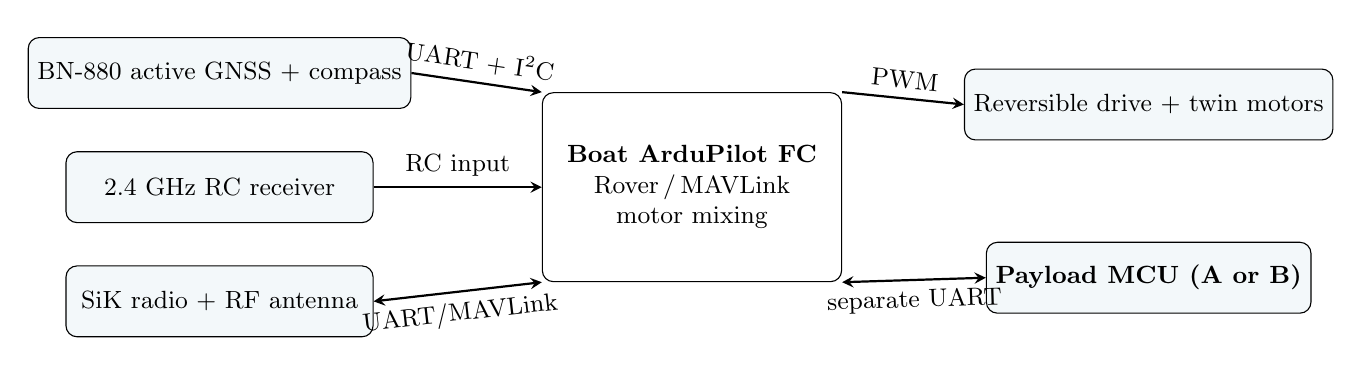
\begin{tikzpicture}[>=stealth,every node/.style={font=\small},node distance=3mm]
\node[draw,rounded corners,fill=pale,minimum width=39mm,minimum height=9mm] (gnss) at (0,2.0) {BN-880 active GNSS + compass};
\node[draw,rounded corners,fill=pale,minimum width=39mm,minimum height=9mm] (rc) at (0,0.55) {2.4 GHz RC receiver};
\node[draw,rounded corners,fill=pale,minimum width=39mm,minimum height=9mm] (rf) at (0,-0.9) {SiK radio + RF antenna};
\node[draw,rounded corners,fill=white,minimum width=38mm,minimum height=24mm,align=center] (fc) at (6,0.55) {\textbf{Boat ArduPilot FC}\\Rover\,/\,MAVLink\\motor mixing};
\node[draw,rounded corners,fill=pale,minimum width=40mm,minimum height=9mm] (drv) at (11.8,1.6) {Reversible drive + twin motors};
\node[draw,rounded corners,fill=pale,minimum width=40mm,minimum height=9mm] (payload) at (11.8,-0.6) {\textbf{Payload MCU (A or B)}};
\draw[->,thick] (gnss.east) -- node[above,sloped]{UART + I$^2$C} (fc.north west);
\draw[->,thick] (rc.east) -- node[above]{RC input} (fc.west);
\draw[<->,thick] (rf.east) -- node[below,sloped]{UART/MAVLink} (fc.south west);
\draw[->,thick] (fc.north east) -- node[above,sloped]{PWM} (drv.west);
\draw[<->,thick] (fc.south east) -- node[below,sloped]{separate UART} (payload.west);
\end{tikzpicture}\end{center}
\textbf{UART allocation gate:} dedicate one logical serial port to GNSS, one to SiK telemetry and one to payload MCU MAVLink, while RC uses its documented receiver interface. CoreWing's GPS, telemetry, external-compass and RC connectors are documented; \textbf{exact free UART pins, connector voltage and firmware build must be checked on the purchased board} \cite{coreDoc}. MAVLink messages may be dropped, so synchronise timestamps and handle missing observations explicitly \cite{mav}. Use separate antenna positions and isolate high-current motor wiring from compass and RF leads.

\section{Flight-controller comparison and SpeedyBee decision}
\begingroup\footnotesize\begin{tabularx}{\linewidth}{L{31mm}L{34mm}Y L{25mm}}
\toprule \textbf{ECU / purchase} & \textbf{Price, mass and power} & \textbf{Navigation / control evidence} & \textbf{Decision}\\\midrule
CoreWing F405 Wing Mini V2 \cite{coreShop} & \textbf{RM264.43} voucher listing; \SI{19}{g} board-family published figure; 2--6S \cite{coreShop,coreDoc} & ArduPilot Rover board documentation lists GPS, compass, telemetry, receiver, motor outputs and integrated BEC; connector voltage and servo-rail BEC warnings apply \cite{coreDoc}. & \textbf{Preferred in tiers A--C.} UART/pin check required.\\
SpeedyBee F405 V4 \textbf{60A quad ESC stack} \cite{speedShop} & \textbf{RM445.40}; FC: 41.6 $\times$ 39.4 $\times$ 7.8 mm (10.5 g). ESC: 45.6 $\times$ 44 $\times$ 8 mm (23.5 g) \cite{speedDoc} & FC has ArduPilot Rover support, 9 PWM outputs, 6 serial interfaces (some reserved), external I$^2$C compass and microSD \cite{speedAP,speedDoc}. & \textbf{Comparator only.} ESC is quadcopter BLHeli\_S; reversible boat operation \emph{not confirmed}.\\
\bottomrule
\end{tabularx}\endgroup\par\medskip
\textbf{Why not buy the suggested stack first?} The SpeedyBee ESC's \SI{60}{A} channel rating is a \emph{current limit} rather than a motor-power requirement, and its four-channel fixed-wing/quadcopter packaging creates no advantage for a two-motor boat. More importantly, ArduPilot's \emph{bidirectional DShot telemetry} is \textbf{not the same} as physical forward/reverse propulsion; reversal depends on the ESC firmware/mode and motor protocol, and cannot be assumed from the published stack specification \cite{speedDoc,speedAP,motor}. The stack may be retested later but is not costed as a proven reversing drive.

\section{Propulsion and motor-driver technical comparison}
\begin{landscape}
\scriptsize\setlength{\tabcolsep}{2pt}
\begin{longtable}{L{25mm}L{21mm}L{22mm}L{23mm}L{30mm}L{36mm}L{31mm}L{23mm}L{32mm}}
\caption{Motor and driver options: every rating is source-linked; unreported parameters are not inferred. Electrical input is NOT shaft output or horsepower.}\label{tab:motor}\\
\toprule \textbf{Model/channel} & \textbf{Supply} & \textbf{Dimensions} & \textbf{Mass} & \textbf{Thrust / shaft W / hp} & \textbf{Under-load power/current} & \textbf{Max current} & \textbf{Price each} & \textbf{Purchase; technical evidence}\\\midrule\endfirsthead
\toprule \textbf{Model} & \textbf{Supply} & \textbf{Dimensions} & \textbf{Mass} & \textbf{Output} & \textbf{Loaded draw} & \textbf{Current limit} & \textbf{RM ea} & \textbf{Evidence}\\\midrule\endhead
\bottomrule\endfoot
12V three-blade jet unit, Shopee \cite{jetShop} & 12V advertised & NR, sold variant & NR & thrust/shaft W/hp \textbf{NR} & current under water \textbf{NR} & stall/max \textbf{NR} & RM38.50--74.80 variant range; planning \textbf{74.80} & \href{https://shopee.com.my/RC-Boat-12V-Jet-Boat-Underwater-3-blades-Propeller-Motor-Engine-Thruster-for-DIY-RC-ROV-Robot-Bait-Boat-Submarine-i.867757154.29083229097}{Shopee}; no reliable maker sheet; motor type \emph{unconfirmed} \\
Hobbyocean T60 + 40A ESC variations \cite{hobbyShop,hobbyRef} & 12--16V and 2--4S \emph{claimed by third-party spec} & NR for purchased SKU & NR & seller/third-party 300W electrical-rated class; thrust/hp for SKU \textbf{NR} & third-party T60 15--23A \emph{claimed}; no certified curve & ESC 40A \emph{variant claim}; motor limit NR & RM225.98--321.46 variants; \textbf{321.46 A} & \href{https://shopee.com.my/Hobbyocean-Underwater-Thruster-Combo-Brushless-Motor-16V-300W-With-40A-ESC-for-RC-Bait-Tug-Boat-Nest-Ship-Submarin-ROV-Robot-i.487084356.44255991724}{Shopee}; \href{https://www.daraz.com.bd/products/hobbyocean-underwater-thruster-16v-300w-brushless-motor-40a-esc-for-rc-bait-tug-boat-nest-ship-submarin-rov-robot-i571820375.html}{third-party tech, not procurement}; verify \emph{full kit} \\
M060 waterproof BLDC thruster \cite{m060Shop,m060Ref} & 12--24V advertised & \textbf{NR exact SKU} & \textbf{NR exact SKU} & seller variant thrust/shaft W/hp \textbf{NR}; maker-family up-to-3kgf \emph{not transferable} & max-loaded W/A exact SKU \textbf{NR} & max continuous/stall \textbf{NR} & \textbf{273.32}, voucher listing & \href{https://shopee.com.my/M060-200m-Deepwater-Thruster-Waterproof-Brushless-DC-Motor-ROV-Propulsor-12V-24V-Parts-for-RC-Unmanned-Ship-Underwater-Robot-i.133237764.45758558847}{Shopee}; \href{https://fulldepthrov.en.made-in-china.com/product/NAMpUOYlXFRr/China-M060-3kg-Max-Small-Compact-Thrust-Underwater-Brushless-Thruster-for-Underwater-Robot-Rov-Auv-Uuv.html}{manufacturer-family reference} \\
Cytron MDD10A, \emph{brushed only} \cite{mdd10} & 5--30V motor & \mbox{84.5$\times$ 62\,mm} \cite{mdd10} & NR & n/a (H-bridge driver) & loss/heat case-specific & \textbf{10A continuous / channel}, check product manual; 2 channels & \textbf{108.78} & \href{https://my.cytron.io/c-motor-driver/c-dc-motor-driver/p-10amp-5v-30v-dc-motor-driver-2-channels}{Cytron}; NOT direct RC pulse input \\
Cytron MDD3A, \emph{brushed only} \cite{mdd3} & 4--16V motor & NR & NR & n/a & current load user-dependent & \textbf{3A continuous / channel, 5A peak}; 2 channels & \textbf{39.06} & \href{https://my.cytron.io/c-motor-driver/c-dc-motor-driver/p-3amp-4v-16v-dc-motor-driver-2-channels}{Cytron}; \emph{not} safely sized without motor current \\
ZTW Shark G2 20A reversible ESC \cite{ztwShop,ztwDoc} & 2--4S advertised for 20A family & maker data for one variant; sold SKU NR & NR sold SKU & n/a; supports BLDC only & loss/thermal draw \textbf{NR} & 20A \emph{nominal selected variant}, actual motor matching unproven & \textbf{100.00 A}, seller listing RM67.65--227.70 & \href{https://shopee.com.my/ZTW-Shark-G2-20A-30A-40A-50A-60A-80A-100A-2-4S-2-6S-32-bit-Water-cooling-Dual-way-Waterproof-Brushless-ESC-For-RC-Boat-underwater-Thruster-i.53025383.19459335204}{Shopee}; \href{https://www.ztwoem.com/products/info.html?id=157}{OEM family page} \\
\end{longtable}
\end{landscape}
\textbf{Motor-drive incompatibility gates.} Tier A may use MDD10A \emph{only after} a two-wire brushed motor is positively identified, its submerged load is measured below the channel limit and the controller input is translated into PWM/direction. BLDC motors require BLDC ESCs, not MDD10A. Tiers B and C require confirmed bidirectional 3S operation, independent PWM inputs, waterproof cabling, current limits and CW/CCW propeller arrangements. Voltage $\times$ current is \emph{electrical input}; no horsepower figure can be honestly assigned without torque/rpm or shaft-dynamometer data.

\section{Active GNSS, RC, telemetry and battery comparison}
\small
\begin{longtable}{L{29mm}L{29mm}L{48mm}L{18mm}L{36mm}}
\caption{Separate functions and technical evidence. Published values are attributed row by row.}\label{tab:other}\\
\toprule \textbf{Item} & \textbf{Electrical/physical} & \textbf{Interfaces, benefits and caveats} & \textbf{RM ea} & \textbf{Sourcing/evidence}\\\midrule\endfirsthead
\toprule \textbf{Item} & \textbf{Envelope/power} & \textbf{Evidence} & \textbf{RM} & \textbf{Source}\\\midrule\endhead\bottomrule\endfoot
Beitian BN-880 \emph{active GNSS patch} + compass \cite{bnShop,bnData,bnMaker} & \mbox{28$\times$ 28$\times$ 10\,mm}, approx \SI{10}{g}; 3--5.5V family, 50mA capture typical (secondary docs) & Integrated active GNSS patch and I$^2$C compass claimed; serial GNSS output, compass on separate lines; vendor/board revision identification required & 118.42 voucher & \href{https://shopee.com.my/Beitian-BN-880-Flight-Control-GPS-Module-Dual-Module-Compass-With-Cable-i.23419821.885903382}{Shopee}; \href{https://store.beitian.com/it/blogs/news/gps-modules-with-arduino-and-raspberry-pi}{maker}; \href{https://manuals.plus/ae/1005008660355732}{datasheet mirror}\\
GI separate \emph{active} GPS antenna \cite{activeShop} & \SI{26}{dB} gain; \SI{50}{\ohm}; \SI{18}{mA} typical; 3m cable & SMA/IPX cable supplied; \textbf{requires compatible active-antenna RF receiver + bias}; \emph{do not} connect to BN-880 by assumption & 27.00 & \href{https://www.gie.com.my/shop.php?action=wireless/gps/gps_active_ant}{GI Electronic}; receiver extra, not costed\\
M10 + IST8310 GNSS/compass \cite{m10Shop} & exact antenna active/passive \textbf{NR}; mass/size NR & Alternate GNSS, but does \emph{not} satisfy active-antenna requirement until antenna/LNA confirmed; cable pinout must be checked & 125.09 voucher & \href{https://shopee.com.my/M10-GPS-Module-With-External-IST8310-Compass-For-Pixhawk-2.4.8-PIXRACER-R15-RC-Quadcopter-Plane-Drone-RC-Boat-RC-Upgrade-Parts-i.487084356.42854127762}{Shopee}\\
HotRC 6ch \SI{2.4}{GHz} RC Tx + Rx \cite{hotrc} & Tx \SI{230}{g}; receiver 4--9V; receiver mass NR & Six RC channels, fail-safe listed; packet protocol/receiver output interface confirm; as checked on 5 Nov backorder & 109.00 & \href{https://my.cytron.io/c-rf-module/p-hotrc-6-channels-rc-radio-transmitter-and-receiver}{Cytron}, transmitter and receiver included\\
FlySky FS-i6X + receiver \cite{flyShop} & 2.4GHz; size/mass exact chosen bundle NR & Alternative if HotRC unavailable; receiver \emph{variant} and compatible iBUS/SBUS to be checked & 207.98 display range example & \href{https://shopee.com.my/FLYSKY-FS-i6X-I6X-AFHDS-2A-RC-Transmitter-with-X6B-IA6B-IA10B-Receiver-10CH-2.4GHz-for-Aairplane-Helicopter-FPV-Racing-Drones-Quadcopter-Multirotor-Free-shipping-i.155465789.25544808687}{Shopee}; displayed entry may not include receiver\\
3DR/SiK \textbf{RF telemetry pair} + antennas \cite{radioShop,radioDoc} & 433/915MHz; listed 100mW--1000mW variants (\emph{not} all selectable at minimum price) & MAVLink over UART to laptop ground radio; compatible TX/RX pair, frequencies and antennas must match; verify local RF rules & \textbf{160.00 A} & \href{https://shopee.com.my/3DR-Radio-Telemetry-433Mhz-915Mhz-100MW-500MW-1000MW-Air-and-Ground-Data-Transmit-Module-with-OTG-for-APM-2.8-Pixhawk-2.4.8-i.756673533.22527872228}{Shopee}: 92.40--462 range, pair price NR; \href{https://docs.ardupilot.org/copter/docs/common-sik-telemetry-radio.html}{ArduPilot}\\
Cytron 3S \SI{2.2}{Ah} LiPo \cite{bat22} & 11.1V nominal; 30C advertised; 24.42Wh \emph{derived} & Testing pack; at 80\% usable, 120-min energy budget $\leq$\SI{9.77}{W} average \emph{(calculation)}, not a runtime claim & 75.00 & \href{https://my.cytron.io/p-lipo-rechargeable-battery-3s-11.1v-30c-2200mah}{Cytron}\\
Cytron 3S \SI{5.2}{Ah} LiPo \cite{bat52} & 11.1V nominal; 30C advertised; \mbox{145$\times$ 45$\times$ 28\,mm}; 57.72Wh \emph{derived} & At 80\% usable, 120-min energy budget $\leq$\SI{23.09}{W} average \emph{(calculation)}; motor draws unknown & 155.00 & \href{https://my.cytron.io/p-lipo-rechargeable-battery-11.1v-5200mah}{Cytron}\\
Shopee XN Eagle 4S 14.8V 4200mAh LiPo \cite{bat4Shopee} & 14.8V nominal, 16.8V fully charged, 55C marketed; dimension and mass for 4S variant NR & 62.16Wh nominal derived; at 80\% usable, 120-min overall average $\leq\SI{24.86}{W}$ (arithmetic only); 4S variant price NOT isolated from 2S--6S dropdown & 174.67 \emph{A} & \href{https://shopee.com.my/XN-Eagle-lithium-lipo-battery-4200mah-55c-2s-3s-4s-6s-7.4v-11.1v-14.8v-22.2v-i.10855326.3111591551}{Shopee}; 4S exact SKU and inventory to confirm\\
Cytron B6AC 1--6S balancing charger \cite{charger4} & 100--240VAC or 11--18VDC; max 5A charge; 50W charge power; \SI{575}{g}; 133 by 145 by 35 mm & Balance charges 4S pack on shore; configurable LiPo chemistry, terminal/lead type and safe current must be checked & 95.00 & \href{https://my.cytron.io/p-multi-function-lipo-balance-charger-13853}{Cytron}; maker/distributor specs\\
Cytron 2--3S balance charger \cite{charger} & 110--240V AC, shore-only & Balanced charging, not boat payload; charger model and charging rate must match pack & 19.90 & \href{https://my.cytron.io/p-2-3-cell-lipo-balance-charger}{Cytron}\\
\end{longtable}
\normalsize
\textbf{RF legal/integration gate:} choose the 433 or 915MHz radio variant and configured transmit power only after checking MCMC/SIRIM conditions for intended field use; \emph{no permission or licence exemption is asserted here}. The boat \emph{may} receive waypoints or commands over MAVLink; ACK/HEARTBEAT, link drop-outs and failsafe behaviour need bench and shore trials \cite{radioConfig,radioDoc,mav}. \textbf{Manual override} must remain independent of MAVLink link availability.



\section{Selection rationale: evidence, interfaces and design priorities}
\label{sec:selection}
\textbf{Selection principles.} Minimise electronics mass, reserve one physical port for the payload MCU, keep an independent safety link, use an active GNSS receive front-end, match motor chemistry to battery voltage, and prioritise testable specifications over a low advertised Shopee variant price. The controller must support Rover differential thrust and live MAVLink communications, not merely ``a GPS module and two motors'' \cite{coreDoc,boat,motor,mav}. The 20~m by 20~m, 120-minute mission is a requirement from the project brief, not a performance certificate \cite{project}.

\begin{tabularx}{\linewidth}{L{27mm}Y Y}
\toprule Design decision & Technical justification and cited evidence & Condition for acceptance \\\midrule
CoreWing Mini V2 rather than 60A quad stack & 37$\times$26$\times$14~mm, 19~g; 2--6S input, GPS UART5, I$^2$C compass and Wi-Fi MAVLink; 5V 2A continuous peripheral rail (manufacturer board integration via ArduPilot) \cite{coreDoc}. & Confirm Rover firmware, accessible connector pinout, free serial interfaces and correct ESC PWM output.\\
3S for short dry tests; 4S only with qualified motor & Cytron 3S packs are 11.1~V nominal / 12.6~V charged. Proposed M060 seller family specifies 12--24~V; 4S nominal 14.8~V and charged 16.8~V is within that advertised family range but exact motor variant is still not validated \cite{bat22,bat52,bat4Shopee,m060Shop}. & Test actual battery voltage span, motor current and ESC limit before connection.\\
Two independent radio links & Manual RC permits local takeover; SiK-style telemetry carries two-way MAVLink for mission updates and health data. ArduPilot documents distinct receiver and GCS failsafes \cite{rcDoc,radioDoc,failsafes}. & Prove RC receiver protocol compatibility and separate link-loss actions.\\
Active GNSS + compass & BN-880 supplier variant combines GNSS antenna, UART position and compass interface; CoreWing provides UART5 + I$^2$C but not onboard GNSS \cite{bnShop,bn880Series,coreDoc}. & Verify active patch physically, wiring, outdoor GPS fix and magnetic installation.\\
Two pontoon tubes & Nominal 110~mm diameter and 1~m length makes a modular light hull candidate; displacement is calculated, not seller-rated cargo capacity \cite{pipe,cap}. & Full-system float, freeboard, static stability and leak tests.\\
\bottomrule
\end{tabularx}

\subsection{Flight controller: why this board and not the more expensive stack?}
The CoreWing F405 Wing Mini V2 uses an STM32F405RGT6 at 168~MHz and integrates a voltage/current monitor, 12 PWM motor/servo outputs, a GPS connector (UART5 plus I$^2$C), telemetry, RC input and an ESP8685 wireless interface. ArduPilot specifies 2--6S input (7--28~V), a 5~V / 2~A continuous peripheral BEC and a 5/6~V servo BEC rated 4~A continuous for the Mini V2 \cite{coreDoc}. These are \emph{board ratings}, not overall ship-load ratings. Its 19~g mass and 37$\times$26$\times$14~mm size reduce the electronics packaging penalty compared with a larger board \cite{coreDoc}. The cited Shopee price remains variant-dependent \cite{coreShop}.

For reference, the SpeedyBee F405 V4 60A stack has a manufacturer-documented FC plus four-channel quad ESC, but neither a 60~A ESC rating nor support for ArduPilot entails reversible propulsion. A differential-drive boat needs two motors that can physically reverse and whose ESCs interpret the Rover control signal correctly. The included quad ESC was therefore \textbf{not} used as a verified replacement for two reversible marine ESCs \cite{speedDoc,speedAP,motor}. \textbf{Firmware gate:} flash the board-specific Rover target and confirm firmware memory-feature limitations before purchasing optional sensors \cite{coreDoc}.

\subsection{Proposed port and power allocation (pinout to be checked on actual board)}
\begin{tabularx}{\linewidth}{L{34mm}L{45mm}Y}
\toprule Device & Suggested FC connection & Why / gate \\\midrule
Active BN-880 GNSS & GPS1 on UART5; compass SDA/SCL on I$^2$C & CoreWing manufacturer integration explicitly assigns GPS UART5 and shared I$^2$C. Verify TX/RX crossing, pin order and 4V5 supply \cite{coreDoc,bn880Series}.\\
Independent RC receiver & Dedicated SBUS/PPM or supported serial RC on UART6 & \textbf{Not the individual PWM pins of the HotRC receiver unless a supported PPM encoder is included.} Verify actual protocol, failsafe and receiver supply voltage \cite{coreDoc,hotrcCurrent,rcPWMEncoder}.\\
SiK UART telemetry & Candidate SERIAL4 / UART4 (after pin access check) & Configure a MAVLink serial protocol and supported baud rate. Board labels and physical harness must be confirmed \cite{coreDoc,radioConfig}.\\
Payload MCU & Candidate SERIAL3 / UART3 (after pin access check) & Physically separate MCU, short protected serial cable, common signal reference or isolation as required, MAVLink position/time/status transfer \cite{coreDoc,mav}.\\
Built-in Wi-Fi & SERIAL1 tied to wireless module & Used only as alternative development telemetry; it does not remove GPS, RC or payload MCU port needs \cite{coreDoc}.\\
Twin reversible ESCs & Two PWM-capable servo outputs & Set Rover skid-steer mixing, neutral deadband, reverse direction and failsafe outputs; do not confuse bidirectional DShot \emph{telemetry} with propeller reversal \cite{coreDoc,motor,ztwDoc}.\\
\bottomrule
\end{tabularx}

\textbf{Power-rail and noise check.} CoreWing warns that its servo rail already has an onboard BEC; connecting a marine ESC's BEC red wire without checking board jumpers can backfeed supplies. The board also recommends a 35~V, 470~\si{\micro\farad} capacitor on battery input to reduce switching noise affecting its current monitor \cite{coreDoc}. Do not assume the Mini's regulated 5~V rail can supply an unknown payload computer: the payload MCU has an independent power budget. Battery current sensing must be calibrated with a meter. A power distribution design must separately size motor-circuit fuses, ESC wiring, FC supply and grounds \cite{coreDoc,fuse,wire}.

\section{Battery selection: voltage, energy and realistic endurance}
\label{sec:battery}
\subsection{What the supplier actually specifies}
The registered Cytron listings state that both proposed 3S LiPo batteries have 11.1~V nominal voltage, 12.6~V at full charge and a marketed 30C discharge rating. The 2.2~Ah battery measures 105$\times$33$\times$21~mm and costs RM75; the 5.2~Ah battery measures 145$\times$45$\times$28~mm and costs RM155. \emph{Neither listing provides a validated mass, internal-resistance curve or field discharge profile} \cite{bat22,bat52}. Cytron warns these packs have no built-in protection against short circuits and need dedicated LiPo charging \cite{bat22,bat52}.

The Shopee XN Eagle 4S option is advertised as 14.8~V nominal, 4.2~Ah and 55C, but it is a \textbf{multi-variant listing}: exact 4S mass, dimensions, connector and final price must be obtained from the selected checkout variant. The current RM174.67 is still a \textbf{planning allowance}, not a manufacturer-verified quote \cite{bat4Shopee}. A 4S LiPo reaches 16.8~V fully charged as a cell-count calculation; this is incompatible with an ESC or motor capped at 16.0~V, even if the nominal voltage seems appropriate. Therefore Tier B is barred from 4S connection until the exact T60 version confirms an absolute input rating above the fully charged pack \cite{hobbyShop,hobbyRef}.

\begin{center}\small
\begin{tabularx}{\linewidth}{L{25mm}L{28mm}L{22mm}L{25mm}Y}
\toprule Battery / sourcing & Datasheet/listed values & Nominal energy \emph{(D)} & Max mean W for 2 h \emph{(D)} & Engineering role and caution \\\midrule
Cytron 3S 2.2 Ah \cite{bat22} & 11.1 V, 2.2 Ah, 30C & 24.42 Wh & 9.77 W & Least-cost short bench test; cannot assume 2-h propulsion, GNSS and telemetry.\\
Cytron 3S 5.2 Ah \cite{bat52} & 11.1 V, 5.2 Ah, 30C & 57.72 Wh & 23.09 W & Better capacity, but insufficient verified operating voltage for nominal 12--24 V underwater thrusters.\\
Shopee 4S 4.2 Ah \cite{bat4Shopee} & 14.8 V, 4.2 Ah, advertised 55C & 62.16 Wh & 24.86 W & Only candidate 4S pack after variant verification; T60 16 V limit remains unresolved.\\
\bottomrule
\end{tabularx}
\end{center}
The energy values are derived by $E_{\mathrm{nom}}=V_{\mathrm{nom}}C$ using nominal voltage and ampere-hours from cited supplier pages. The mean-power limits use the explicit \emph{engineering assumption} that 80\% of nominal energy is available to the boat throughout a two-hour mission:
\[
  P_{\mathrm{mean,max}}=\frac{0.8\, V_{\mathrm{nom}} C}{2\ \mathrm{h}}.
\]
This is not a measured state-of-health correction, weather reserve, or a guarantee of two-hour operation. With a 4S 4.2~Ah pack, a measured \emph{total} boat draw of 10, 20, 25 or 40~W would give idealised runtimes of 4.97, 2.49, 1.99 or 1.24~h respectively under this 80\% assumption; actual performance needs a discharge test at the load profile \cite{bat4Shopee}.

\subsection{Why capacity, C-rating and peak motor current are separate criteria}
The advertised 30C ratings mathematically imply $30\times2.2=66$~A and $30\times5.2=156$~A; the Shopee 55C/4.2~Ah label mathematically implies 231~A. \textbf{These are marketing-derived theoretical figures, not tested allowable continuous currents} and do not replace cell temperature, connector, cable, fuse or ESC limits \cite{bat22,bat52,bat4Shopee}. The design current must come from the \emph{actual submerged motor load}, including turning and transient acceleration, plus controllers, radios and payload-interface electronics.\par
\textbf{Sizing sequence.} First measure cruise, turn, start and static-maximum currents for each propeller/ESC combination at the intended immersion. Then log $P(t)=V(t)I(t)$ and integrate $\int_0^{7200\,\mathrm{s}}P(t)\,dt$ to estimate mission Wh. Add return-to-shore reserve and battery ageing margin. Choose the pack only after the measured maximum demand and mission energy both fit the pack \emph{and} voltage range. The initial 2-hour gate should fail if only calculated nominal Wh are presented \cite{project,failsafes}.\par
\textbf{Charging/safety selection.} The RM19.90 Cytron 2--3S charger is suitable only for relevant 2--3-cell chemistries, so it cannot charge a 4S battery \cite{charger}. The RM95 Cytron B6AC permits 1--6 LiPo cells, 0.1--5.0~A setting and a 50~W maximum charge rate, which makes it a compatible class of \emph{shore charger} for a verified 4S pack, subject to correct balance lead, charge chemistry and current setting \cite{charger4}. Set up battery monitoring and tested low-voltage/current failsafes, including a physical isolation switch and branch fuses; ArduPilot's low-voltage/capacity failsafes require accurate battery measurements \cite{coreDoc,failsafes,kill,fuse}.

\section{Active GPS and antenna selection: reception is not navigation accuracy}
\label{sec:gps}
\subsection{BN-880: reason for selecting a combined module}
The listed BN-880 combines a GNSS receiver, antenna patch and magnetic compass in one small housing, saving a separate receiver/antenna/compass assembly. The BN-880-series pinout identifies six connections: compass SDA/SCL, GNSS TX/RX, supply and ground; hence it can connect directly in \emph{interface terms} to CoreWing UART5 plus I$^2$C, with the exact connector/harness confirmed before power-up \cite{bnShop,bn880Series,coreDoc}. A reproduced BN-880 specification reports approximately 28$\times$28$\times$10~mm, approximately 10~g in one reseller listing, a nominal 5~V supply and approximately 50~mA acquisition draw at 5~V; $5(0.05)=0.25$~W is a \emph{derived upper-level planning figure}, not an independent consumption measurement \cite{bn880Secondary,bn880Series}. The listing's \emph{active-antenna} assertion must be checked against the actual module label/circuit, since Shopee variations and unofficial reproductions do not constitute traceable manufacturer testing \cite{bnShop,bnData}.

For technical provenance, Beitian's \emph{official} BE-880 (note the extra letter ``E'': \textbf{not the BN-880 SKU}) is published at 28$\times$28$\times$11~mm, 12~g, 3.6--5.5~V and 15~mA typical at 5~V using an M10050 receiver. Those numbers \emph{must not be transferred to BN-880} without confirming the received device is actually the BE-880 \cite{beitianOfficialBE}. This comparison demonstrates why the report states model and revision rather than copying attractive GNSS numbers between different Beitian products.

\subsection{Antenna options and why adding ``26 dB'' is not automatic improvement}
\begin{tabularx}{\linewidth}{L{32mm}L{39mm}Y}
\toprule Approach & Traceable evidence & Suitability / risk \\\midrule
Integrated BN-880 patch (baseline) & Shopee GNSS/compass listing and BN-880-series pinout; antenna amplification asserted, not independently RF-tested \cite{bnShop,bnData,bn880Series}. & Compact, few connectors, low cable loss; mount with clear sky view above splashes and away from high-current motor wiring.\\
GI K0500001 separate active antenna & Registered supplier specifies RM27, 26~dB advertised gain, 50~$\Omega$ output, 18~mA typical current, 3~m cable and IPX--SMA adapter \cite{activeShop}. & Requires a \emph{different compatible GNSS receiver} with active-antenna bias and matching RF connector; not electrically connectable to a sealed BN-880 by assumption.\\
Shopee M10 + IST8310 compass & Seller lists M10 receiver with external compass but does not substantiate active antenna/LNA, receiver/antenna gain, cable or exact mass for a chosen variant \cite{m10Shop}. & Only qualify if maker documents active RF front-end and actual received board; not an automatic substitute for mandatory active GNSS.\\
\bottomrule
\end{tabularx}

A ``26~dB'' advertised antenna gain does \emph{not} establish final GPS accuracy or range: the receiver must supply suitable antenna bias, impedance must match, and a 3~m feed adds frequency-dependent loss. The GI listing provides no matched-receiver validation, waterproof connector rating, or \emph{system-level} accuracy test \cite{activeShop}. The separate antenna is therefore an option for a properly designed receiver front-end, not a budget line that can simply be added to the BN-880.

\subsection{GNSS performance requirement for a 20 by 20 m grid}
The BN-880 secondary specifications describe approximately 2~m horizontal position accuracy under favourable open-sky assumptions \cite{bn880Secondary}; Beitian's separate official BE-880 lists 2.0~m CEP, but again this is \emph{different hardware} \cite{beitianOfficialBE}. The project uses 5~m nominal lane separation as an engineering planning value. On a compact surface boat, multipath from banks, compass errors, crosswind and finite control response may consume the spacing margin, so \textbf{5~m repeatable lane accuracy has not been demonstrated} by the module's nominal figure alone. Compass readings must be calibrated with thrusters on and off; motor and ESC interference is a recognised reason that ArduPilot supports dual-GNSS yaw alternatives \cite{gpsYaw}.\par
\textbf{Acceptance test:} log GNSS fix quality, horizontal dilution/accuracy estimator, compass heading, ground-track cross-track error, and repeated waypoint returns for multiple directions. Keep time-stamped raw logs and compare against marked shore reference points; if the resulting cross-track distribution erases coverage, change spacing or upgrade positioning before claiming full spatial coverage. The boat FC passes timestamped position and fix metadata to the separate payload MCU; GNSS hardware is \emph{not} part of the payload budget \cite{coreDoc,mav,project}.

\section{Radio modules and antennas: three independent jobs}
\label{sec:radio}
\subsection{Manual RC: why it remains mandatory even with autonomy}
The Cytron HotRC kit includes a transmitter and receiver and lists 2.4~GHz FHSS, six channels, 4--9~V receiver power, PWM response at or below 20~ms, approximately 230~g \emph{transmitter mass}, and advertised 300~m ground/800~m air distances \cite{hotrcCurrent}. The distances are supplier marketing values, \textbf{not a measured over-water range}. A six-channel link is useful for steering, throttle, mode selection and an independent stop; the exact channel assignments are configuration choices \cite{rcDoc,failsafes}.

\textbf{Critical compatibility correction to V3.1.} Cytron does \emph{not} establish that the HotRC receiver exports a combined SBUS, PPM or compatible serial protocol. A 6-channel \emph{individual PWM} receiver does not plug into CoreWing's single SBUS/PPM input as if it were one combined control stream. ArduPilot explicitly describes PPM encoders for old-style parallel PWM receivers \cite{hotrcCurrent,coreDoc,rcPWMEncoder}. \textbf{Purchase gate:} request the receiver model/pinout and confirm a single combined signal, or add a registered-supplier/Shopee-sourced encoder and its price, or select a transmitter + receiver bundle with documented compatible serial output. Until then the RC part and hence every displayed tier subtotal is conditional. The Shopee FlySky alternative has transmitter/receiver variants; a price for \emph{transmitter only} must not be used as the price of an operable RC link \cite{flyShop,rcProtocols}.

\subsection{RF telemetry: why SiK rather than using the RC channels for everything?}
For ground-station status, waypoints and parameter changes, use a transparent two-way serial channel carrying MAVLink. ArduPilot's SiK reference describes small radio modems in 433 and 915~MHz variants, under 4~g \emph{without antenna}, up to 20~dBm / 100~mW in the documented reference platform, sensitivity down to -121~dBm and configurable serial/air data rates (up to 250~kbit/s) \cite{radioDoc}. These are \emph{reference-platform} specifications, \textbf{not} verified performance or frequency approval for the selected Shopee 100/500/1000~mW multi-variant listing \cite{radioShop}. The boat unit needs a UART, regulated compatible power and antenna; the ground unit needs a matched antenna and USB interface to Mission Planner \cite{radioDoc,radioConfig}.\par
In a 20 by 20~m test area, onboard CoreWing Wi-Fi can carry TCP/UDP MAVLink without additional RF hardware \cite{coreDoc}; this saves the provisional RM160 SiK-pair allowance. However, no board-specific Wi-Fi antenna gain, water-level propagation plot, outdoor packet-loss rate or link range is published in the cited board documentation. Wi-Fi is a \emph{development alternative}, not proof of a robust survey control link. Retain RC manual override regardless \cite{coreDoc,failsafes}.\par
\textbf{Antenna bill of materials:} one antenna on the RC \emph{receiver} and its matching transmitter aerial (normally bundled), plus one antenna per SiK radio at the boat and shore. The exact Shopee radio purchase must explicitly include \emph{two modems, two correct-band antennas, USB/UART cable and connectors} or the cost table must add missing items. Do not interchange 433 and 915~MHz antennas, infer gain or range from their appearance, or assume the seller's high-power option shares the ArduPilot 100~mW reference characteristics \cite{radioDoc,radioShop}. The correct Malaysian frequency band and transmit power require a documented MCMC/SIRIM compliance check before deployment; this report does not claim approval.\par
\textbf{Placement rationale:} position GNSS patch facing the sky; stand RC/RF aerials clear of water, battery and conductive motor wiring; route power cables together and separate them from the compass lead where physically practical. These are noise-reduction design decisions that need a field link-budget and compass-disturbance test; no numerical radio-range claim follows from these recommendations \cite{gpsYaw,coreDoc,radioDoc}.

\subsection{Loss-of-link behaviour: a safety case, not a checkbox}
ArduPilot distinguishes RC receiver loss from ground-station MAVLink heartbeat loss. The Rover documentation gives a default RC timeout of 1~s and default GCS heartbeat timeout of 5~s; neither default should be taken as a verified safe action. A lost RC link may result in Hold, RTL or Disarm according to parameters, while GCS loss may cause a different behaviour \cite{failsafes}. \textbf{Dry-test each combination} of RC loss, telemetry loss, GPS unavailable and low battery; only allow autonomous motion when the independently testable chosen response is safe for the environment. Hardware kill-switch operation remains separate from these software failsafes \cite{failsafes,kill}. \textbf{Do not advertise RC as a guaranteed emergency stop} until observed receiver failsafe output and ArduPilot modes have been tested.

\section{Propulsion, waterproofing and small components: justification ledger}
\label{sec:auxiliary}
\begin{longtable}{L{40mm}L{78mm}L{44mm}}
\caption{Why each remaining boat-common component is included; product figures are source-linked, and selection gaps remain explicit.}\label{tab:justledger}\\
\toprule Component & Engineering reason for including it & Required evidence / unresolved qualification \\\midrule\endfirsthead
\toprule Component & Reason & Acceptance test \\\midrule\endhead\bottomrule\endfoot
Two underwater motors and propellers \cite{jetShop,hobbyShop,m060Shop} & Differential thrust makes turning possible without a separate rudder servo, and provides independent port/starboard actuation with Rover motor mixing \cite{boat,motor}. & Verify motor type, both directions, CW/CCW propeller geometry, thrust at cruise, wet current, seals.\\
Cytron MDD10A (Tier A only) \cite{mdd10} & Dual brushed motor driver; 5--30~V motor input, 10~A continuous and 30~A / 10~s per channel; 84.5$\times$62~mm. Useful only if the two-wire motors are brushed. & Motor type and peak current; \textbf{PWM/DIR is not RC-servo PWM}. Include verified interface translation.\\
T60 kit ESC (Tier B) \cite{hobbyShop,hobbyRef} & Intended integrated BLDC drive concept, but listing variants may be bare motor, ESC or bundle. ``300~W'' is not proof of shaft power or 120-minute cruise load. & Exactly sold variant, reverse firmware, 4S fully charged voltage, heat/current test.\\
ZTW Shark G2 20~A ESC (Tier C) \cite{ztwDoc,ztwShop} & OEM specifies 20~A continuous / 30~A burst, 2--4S, 60$\times$33$\times$10~mm, 32~g and adjustable 5/6~V, 4~A BEC. Reversible marine BLDC alternative. & Verify 20~A exact seller SKU, wet M060 current $<20$~A continuous, separate ESC BEC red lead, thermal response.\\
CoreWing board built-in regulator \cite{coreDoc} & Supplies lightweight boat navigation electronics, reducing external conversion boards in early prototypes. & Track 5~V peripheral current vs 2~A board rating; prevent servo BEC backfeeding.\\
LiPo charger \cite{charger,charger4} & Enables supervised cell-balanced shore charging; 4S build needs a 1--6S unit, not a 2--3S charger. & Match battery connector, balance port, chemistry and configured current.\\
UPVC pontoons and end caps \cite{pipe,cap} & Modular float tubes with a nominal cylindrical displacement; twin geometry offers initial transverse stability and a platform between floats. & Verify actual pipe OD, cap fit, total mass, freeboard, yaw stability and leaks.\\
PVC solvent cement \cite{glue} & Seals compatible UPVC cap joints; cheap fastening method with little additional hardware. & Check chemical compatibility, full cure, leak-test without payload.\\
IP65 electronics enclosure \cite{box} & Splash protection and orderly mounting of low-voltage electronics. IP65 is \emph{not} an immersion rating. & Protected deck placement, gasket inspection, cable-gland entry and splash test.\\
Cable glands \cite{gland} & Mechanical sealing and strain relief where cables enter the electronics enclosure. & Choose gland by actual cable diameter, check strain relief and leak path.\\
Fuses and inline holders \cite{fuse} & Protect wiring from damaging fault currents; separate branch fuses prevent one short from bypassing protection. & Choose fuse according to \emph{wire ampacity and measured draw}, not seller's maximum advertised fuse.\\
Wire and connectors \cite{wire} & Electrical distribution between battery, two drivers and avionics; cable cross-section affects loss and overheating. & Do not assume AWG18 is acceptable for motor branches; calculate voltage drop and validate sustained current and connector rating.\\
Manual isolation switch \cite{kill} & Physical battery disconnection during recovery/bench work, independent of software state. & Confirm DC contact rating, wiring, accessible mount and wet-hand operation.\\
\end{longtable}

\section{Acceptance and procurement gates by component}
\label{sec:accept}
\begin{longtable}{L{32mm}L{87mm}L{39mm}}
\caption{Required evidence before paying for a full build or claiming a 120-minute mission.}\label{tab:acceptance}\\
\toprule Subsystem & Minimum test or source document & Current status \\\midrule\endfirsthead
\toprule Subsystem & Pass condition & Status \\\midrule\endhead\bottomrule\endfoot
RC receiver protocol & Seller/manufacturer confirms SBUS/PPM/serial RC on exact bundle; otherwise itemised approved-source PPM encoder, then confirm RC calibration \cite{coreDoc,hotrcCurrent,rcPWMEncoder}. & \textbf{Open: unqualified}.\\
GNSS & Exact variant's active antenna/LNA evidence, 5~V compatibility, UART/I$^2$C pinout, measured GNSS and compass performance \cite{bnShop,bnData,coreDoc}. & Open.\\
Radio pair/antennas & Matched legal-band two-unit SiK kit, boat and ground antennas, cable/connector pinouts and laptop MAVLink command round trip \cite{radioDoc,radioShop}. & Open; RM160 allowance.\\
Battery & Exact pack SKU, weight, connector, charge voltage, thermal and voltage sag, sustained power consumption vs 120-minute objective \cite{bat22,bat52,bat4Shopee}. & Open; 4S price allowance.\\
ESC/propulsion & Correct motor type; reverse enabled; current-vs-thrust bench graph; fully charged pack voltage inside all device ratings \cite{m060Shop,hobbyShop,ztwDoc,mdd10}. & Open; Tier B 16~V conflict.\\
FC power and UART map & Physical harness mapped to manufacturer docs; no ESC BEC rail backfeed; stable GNSS/RC/SiK/payload MCU simultaneous logging \cite{coreDoc}. & Open.\\
Hull, leakage and mass & Weigh assembled system, ballast test with actual payload, freeboard and righting/stability measurement, dry electronics after spray \cite{pipe,box,project}. & Open; no measured displacement.\\
Fail-safe & Physical isolation; deliberately lose RC, SiK/Wi-Fi, GNSS; observe configured Hold/RTL/Disarm; current + voltage monitor under load \cite{failsafes,coreDoc,kill}. & Open.\\
Budget completeness & Quote all exact variants, antenna and RC conversion accessories, wiring, mounts, shipping and charger. & \textbf{Not yet qualified}; the tier totals are partial.\\
\end{longtable}

\section{Three conditional increasing-cost common-core configurations}
\textbf{Voltage engineering correction.} A 3S LiPo is only \SI{11.1}{V} nominal, below the advertised 12V lower bound of the T60 and M060 thruster families. For tiers B/C, replace the original 3S \SI{5.2}{Ah} pack with a \textbf{4S, 14.8V nominal, 4200mAh pack}; a Shopee XN Eagle multi-variant listing spans RM66.67--174.67, so \textbf{RM174.67 is an upper-range \emph{allowance}, not a confirmed 4S price or stocked variant} \cite{bat4Shopee}. Select the Cytron B6AC 1--6S compatible charger, \textbf{RM95} \cite{charger4}, since a 2--3S-only charger \textbf{cannot charge a 4S pack} \cite{charger}. \emph{CRITICAL:} a fully charged 4S LiPo reaches \SI{16.8}{V}; the T60 family sometimes quotes a 16V limit, so the motor supplier \textbf{must confirm full-charge voltage compatibility before 4S is connected} \cite{hobbyRef,hobbyShop}. This remains a design gate, not a proven electrical combination. For M060 12--24V, 4S nominal and charged voltage fall within its advertised range, subject to exact sold-SKU verification \cite{m060Shop}.

\textbf{Important:} These configurations do not vary by sample payload mass. All include two proposed thrusters, an ArduPilot-compatible boat FC, BN-880 \emph{active} GNSS/compass, a \textbf{provisional} RC transmitter/receiver, a bidirectional RF telemetry pair, one LiPo, charger, pontoons, enclosure, fused wiring and isolation switch. \textbf{All tier totals omit any RC PWM-to-PPM encoder or replacement receiver, mounting and missing hardware: none is yet a complete purchase-ready build.} The tier A motor/driver pairing is only a \emph{conditional} study until brushed type and current are confirmed. Tier B pair pricing is a \emph{variant-bounded allowance}, not a verified kit quotation. Tier C ESC prices are allowances. Cost inputs each have purchase references in the complete cost table below.

\begin{tabularx}{\linewidth}{L{17mm}Y Y Y L{18mm}}
\toprule \textbf{Tier} & \textbf{Twin motors / drive} & \textbf{FC, active GPS, radio} & \textbf{Main battery} & \textbf{Rough RM}\\\midrule
A (low) & 2 $\times$ generic 12V underwater jet (\emph{brushed? NR}) + Cytron 2-ch MDD10A \cite{jetShop,mdd10} & CoreWing F405 Mini V2; BN-880 active; HotRC RC; 3DR/SiK pair (A) \cite{coreShop,bnShop,hotrc,radioShop} & 3S 2200mAh \cite{bat22} & \textbf{1192.37}\\
B (mid) & 2 $\times$ T60-type BLDC + 40A reversible ESC bundles \emph{only if verified} \cite{hobbyShop,hobbyRef} & Same common core and antenna/links \cite{coreShop,bnData,hotrc,radioShop} & 4S 4200mAh (A) \cite{bat4Shopee} & \textbf{1751.68}\\
C (upper) & 2 $\times$ M060 12--24V BLDC + 2 $\times$ ZTW 20A ESCs (A) \cite{m060Shop,ztwShop} & Same common core, GPS, RC and RF \cite{coreShop,bnShop,hotrc,radioShop} & 4S 4200mAh (A) \cite{bat4Shopee} & \textbf{1855.40}\\
\bottomrule
\end{tabularx}

\begin{tabularx}{\linewidth}{L{35mm}L{25mm}L{25mm}Y}
\toprule \textbf{Tier total \emph{incl. basic hull}} & \textbf{Remaining vs RM2k} & \textbf{Share of cap} & \textbf{Budget judgement}\\\midrule
A: \textbf{RM 1192.37} & RM 807.63 & 59.6\% & Cheapest \emph{research budget}, but NOT purchase-ready without identifying a brushed/compatible propulsion motor.\\
B: \textbf{RM 1751.68} & RM 248.32 & 87.6\% & \textbf{Conditional only}: confirm T60 motor accepts 16.8V fully charged 4S, ESC variant, and physical forward/reverse.\\
C: \textbf{RM 1855.40} & RM 144.60 & 92.8\% & Very limited remaining headroom; not preferred. Confirm exact motor/ESC variants, peak current and 4S charger.\\
\bottomrule
\end{tabularx}

\textbf{4S budgeting caveat:} Both higher tiers use an estimated 4S 4200mAh price at RM174.67 from a multi-variant Shopee listing. The exact 4S variant may cost less or more and may be unavailable. The old 3S/Cytron B3AC combination is not appropriate for a motor specified to require 12V minimum throughout discharge. \cite{bat4Shopee,charger4,bat52,charger}

\textbf{Additional V3.2 RC gate:} The HotRC bundle is costed but its individual-PWM versus SBUS/PPM/serial output remains unresolved, so a converter or alternative RC bundle could increase every tier cost. Radio pair price and antenna contents remain provisional.\par\medskip\textbf{Critical total caveat:} These are planning subtotals from cited supplier pages and clearly marked allowances. Antenna mounts, correct wiring adapters, watertight fixing hardware, thruster brackets, RF approvals/shipping, propeller guards and final fabrication can change costs; battery and radio variants can change prices. The \textbf{payload MCU, sensors, pumps, filter/flow cell, sample bottles and image processing hardware are excluded}. The 2h gate is \textbf{not proven}. If the RM2,000 ceiling must include payload hardware too, a fresh combined budget is necessary once Track A/B is selected.

\section{Source-audited itemised cost table (per configuration)}
\scriptsize
\begin{longtable}{L{12mm}L{47mm}r r r L{31mm}L{36mm}}
\caption{Common-core cost basis: prices and assumptions attributed by IEEE reference on every row. A = allowance; voucher and variation prices can differ at checkout.}\label{tab:bom}\\
\toprule \textbf{Tier} & \textbf{Purchasable item and source} & \textbf{Qty} & \textbf{RM ea} & \textbf{RM ext} & \textbf{Procurement status} & \textbf{Technical/sourcing caveat}\\\midrule\endfirsthead
\toprule \textbf{Tier} & \textbf{Part/source} & \textbf{Qty} & \textbf{Unit} & \textbf{Ext} & \textbf{Price type} & \textbf{Constraint}\\\midrule\endhead\bottomrule\endfoot
A & CoreWing F405 Wing Mini V2 \cite{coreShop} & 1 & 264.43 & 264.43 & Observed voucher listing & Price for unspecified pin variant; verify Rover firmware \\
A & BN-880 GPS/compass + active patch \cite{bnShop} & 1 & 118.42 & 118.42 & Observed voucher listing & Active patch assertion uses secondary BN-880 datasheet; confirm genuine chip/compass \\
A & HotRC 6ch Tx + Rx bundle \cite{hotrc} & 1 & 109.00 & 109.00 & Published supplier price & Backorder at final check; inspect receiver output protocol before ordering \\
A & 3DR/SiK air+ground radio pair \cite{radioShop} & 1 & 160.00 & 160.00 & PLANNING ALLOWANCE & Visible multi-variant range RM92.40 to RM462; PAIR and exact band NOT verified \\
A & 2-3S LiPo balance charger \cite{charger} & 1 & 19.90 & 19.90 & Published supplier price & Required only if not already available \\
A & IP65 box 263x182x60 mm \cite{box} & 1 & 35.00 & 35.00 & Published supplier price & Water-resistant against jets, NOT watertight on immersion \\
A & 110mm UPVC pipe 1m \cite{pipe} & 2 & 22.90 & 45.80 & Upper listed variant & 100cm each; weight, wall thickness and hull capacity unverified \\
A & 110mm UPVC end cap \cite{cap} & 4 & 5.88 & 23.52 & Observed seller listing & Fit with pipe must be checked \\
A & PVC solvent cement \cite{glue} & 1 & 15.30 & 15.30 & Upper listed variant & Set-up and watertightness tests required \\
A & 10-piece gland kit \cite{gland} & 1 & 7.08 & 7.08 & Upper listed variant & Sizing by actual wire OD \\
A & Fuse holder and fuse \cite{fuse} & 3 & 6.85 & 20.55 & Upper listed variant & Fuse value MUST be set by wire/current ratings \\
A & AWG18 by metre \cite{wire} & 4 & 2.50 & 10.00 & Prior listing, re-quote & Not necessarily suitable for high-current motor branches \\
A & 12-48V battery isolator \cite{kill} & 1 & 29.99 & 29.99 & Observed seller listing & Seller 275A claim unverified; confirm contact ratings \\
A & 12V 3-blade underwater jet thruster \cite{jetShop} & 2 & 74.80 & 149.60 & Upper visible variant / NOT MOTOR-SPECIFIC & Brushed/BLDC type, stall draw, CW and CCW pair unconfirmed \\
A & Cytron MDD10A 2ch brushed H-bridge \cite{mdd10} & 1 & 108.78 & 108.78 & Published supplier price & ONLY if motor is confirmed brushed and each channel <= 10A continuous \\
A & 3S 11.1V 2200mAh LiPo \cite{bat22} & 1 & 75.00 & 75.00 & Published supplier price & Short-duration bench/RC testing only; 2h not established \\
B & CoreWing F405 Wing Mini V2 \cite{coreShop} & 1 & 264.43 & 264.43 & Observed voucher listing & Price for unspecified pin variant; verify Rover firmware \\
B & BN-880 GPS/compass + active patch \cite{bnShop} & 1 & 118.42 & 118.42 & Observed voucher listing & Active patch assertion uses secondary BN-880 datasheet; confirm genuine chip/compass \\
B & HotRC 6ch Tx + Rx bundle \cite{hotrc} & 1 & 109.00 & 109.00 & Published supplier price & Backorder at final check; inspect receiver output protocol before ordering \\
B & 3DR/SiK air+ground radio pair \cite{radioShop} & 1 & 160.00 & 160.00 & PLANNING ALLOWANCE & Visible multi-variant range RM92.40 to RM462; PAIR and exact band NOT verified \\
B & Cytron 1--6S multifunction balance charger \cite{charger4} & 1 & 95.00 & 95.00 & Published supplier price & 4S-capable shore charger, matching connector required \\
B & IP65 box 263x182x60 mm \cite{box} & 1 & 35.00 & 35.00 & Published supplier price & Water-resistant against jets, NOT watertight on immersion \\
B & 110mm UPVC pipe 1m \cite{pipe} & 2 & 22.90 & 45.80 & Upper listed variant & 100cm each; weight, wall thickness and hull capacity unverified \\
B & 110mm UPVC end cap \cite{cap} & 4 & 5.88 & 23.52 & Observed seller listing & Fit with pipe must be checked \\
B & PVC solvent cement \cite{glue} & 1 & 15.30 & 15.30 & Upper listed variant & Set-up and watertightness tests required \\
B & 10-piece gland kit \cite{gland} & 1 & 7.08 & 7.08 & Upper listed variant & Sizing by actual wire OD \\
B & Fuse holder and fuse \cite{fuse} & 3 & 6.85 & 20.55 & Upper listed variant & Fuse value MUST be set by wire/current ratings \\
B & AWG18 by metre \cite{wire} & 4 & 2.50 & 10.00 & Prior listing, re-quote & Not necessarily suitable for high-current motor branches \\
B & 12-48V battery isolator \cite{kill} & 1 & 29.99 & 29.99 & Observed seller listing & Seller 275A claim unverified; confirm contact ratings \\
B & Hobbyocean T60-type 16V BLDC + 40A ESC bundle \cite{hobbyShop} & 2 & 321.46 & 642.92 & Upper visible variant / BUNDLE UNCERTAIN & Seller variants may be motor-only/ESC-only; forward/reverse must be confirmed \\
B & 4S 14.8V 4200mAh LiPo \cite{bat4Shopee} & 1 & 174.67 & 174.67 & Upper listed variant / ALLOWANCE & Exact 4S price and inventory NR; 4S charged is 16.8V; verify thruster/ESC limits \\
C & CoreWing F405 Wing Mini V2 \cite{coreShop} & 1 & 264.43 & 264.43 & Observed voucher listing & Price for unspecified pin variant; verify Rover firmware \\
C & BN-880 GPS/compass + active patch \cite{bnShop} & 1 & 118.42 & 118.42 & Observed voucher listing & Active patch assertion uses secondary BN-880 datasheet; confirm genuine chip/compass \\
C & HotRC 6ch Tx + Rx bundle \cite{hotrc} & 1 & 109.00 & 109.00 & Published supplier price & Backorder at final check; inspect receiver output protocol before ordering \\
C & 3DR/SiK air+ground radio pair \cite{radioShop} & 1 & 160.00 & 160.00 & PLANNING ALLOWANCE & Visible multi-variant range RM92.40 to RM462; PAIR and exact band NOT verified \\
C & Cytron 1--6S multifunction balance charger \cite{charger4} & 1 & 95.00 & 95.00 & Published supplier price & 4S-capable shore charger, matching connector required \\
C & IP65 box 263x182x60 mm \cite{box} & 1 & 35.00 & 35.00 & Published supplier price & Water-resistant against jets, NOT watertight on immersion \\
C & 110mm UPVC pipe 1m \cite{pipe} & 2 & 22.90 & 45.80 & Upper listed variant & 100cm each; weight, wall thickness and hull capacity unverified \\
C & 110mm UPVC end cap \cite{cap} & 4 & 5.88 & 23.52 & Observed seller listing & Fit with pipe must be checked \\
C & PVC solvent cement \cite{glue} & 1 & 15.30 & 15.30 & Upper listed variant & Set-up and watertightness tests required \\
C & 10-piece gland kit \cite{gland} & 1 & 7.08 & 7.08 & Upper listed variant & Sizing by actual wire OD \\
C & Fuse holder and fuse \cite{fuse} & 3 & 6.85 & 20.55 & Upper listed variant & Fuse value MUST be set by wire/current ratings \\
C & AWG18 by metre \cite{wire} & 4 & 2.50 & 10.00 & Prior listing, re-quote & Not necessarily suitable for high-current motor branches \\
C & 12-48V battery isolator \cite{kill} & 1 & 29.99 & 29.99 & Observed seller listing & Seller 275A claim unverified; confirm contact ratings \\
C & M060 underwater BLDC thruster 12-24V \cite{m060Shop} & 2 & 273.32 & 546.64 & Observed voucher listing, 2 variants & No validated thruster input draw or thrust for exact variant \\
C & ZTW Shark G2 20A bidirectional ESC \cite{ztwShop} & 2 & 100.00 & 200.00 & PLANNING ALLOWANCE & Listing RM67.65-227.70 over all variants; 20A exact not quoted; motor <=20A unproven \\
C & 4S 14.8V 4200mAh LiPo \cite{bat4Shopee} & 1 & 174.67 & 174.67 & Upper listed variant / ALLOWANCE & Exact 4S price and inventory NR; 4S charged is 16.8V; verify thruster/ESC limits \\
\end{longtable}
\normalsize
\section{Mass, energy, buoyancy and validation gates}
The hull concept reuses two \SI{110}{mm} nominal-diameter \SI{1}{m} UPVC pontoons, end-capped and solvent-bonded \cite{pipe,cap,glue}. \textbf{Ideal external cylindrical displacement} (not verified load capacity) is $V_{\mathrm{ext}}=2\pi (0.055\,\mathrm{m})^2 (1.0\,\mathrm{m})=\SI{19.0}{L}$, calculated using the listed nominal diameter and nominal length; real waterplane, wall thickness, caps, freeboard and stability \emph{reduce the usable margin}. At half immersion the simplistic submerged volume is approximately \SI{9.5}{L}, so it is unsafe to infer \SI{9.5}{kg} useful payload: \emph{the entire boat mass} consumes this displacement. The V3 Method Rationale's stored-water scenarios cannot be assigned to this hull without a redesigned float geometry and direct flotation testing.

For 120-min operation, the new Tier B/C \SI{4.2}{Ah} 4S pack has $14.8\,\mathrm{V}\times4.2\,\mathrm{Ah}=\SI{62.16}{Wh}$ nominal (derived from the advertised cell count and capacity) \cite{bat4Shopee}. If the \emph{engineering assumption} is that only 80\% of nominal energy is usable, the entire boat load must average $\leq 62.16\times0.8/2\approx\SI{24.86}{W}$ to operate for \SI{2}{h}, \emph{without weather/current margin}. The Tier A \SI{2.2}{Ah} 3S pack similarly provides only $11.1\times2.2=\SI{24.42}{Wh}$ nominal, or $24.42\times0.8/2=\SI{9.77}{W}$ over two hours \cite{bat22}. These are \textbf{battery-only arithmetic constraints}, not measured endurance. Motor load curves and bridge efficiency remain unknown \cite{jetShop,hobbyShop,m060Shop}. Two independent 3S packs are \emph{not} assumed to be safely paralleled.

\textbf{Pass/fail gates before any full-water trial:}
\begin{enumerate}[leftmargin=*,itemsep=2pt]
\item \textbf{Procurement:} prove correct purchased motor CW/CCW variants, brush type, driver mode, ESC kit inclusion and exact checked-out price; verify RC receiver and air/ground radio pair include antennas.
\item \textbf{Dry electronics:} test 3S powered flight controller, active GNSS fix, compass away from thruster leads, independent RC disarm and MAVLink ground-station mode/waypoint command.
\item \textbf{Power protection:} check wire and fuse ratings; test battery isolator, BEC topology, common grounds, telemetry pins and potential ESC BEC backfeed.
\item \textbf{Waterproofing:} static leak test, float/freeboard and full-mass stability tests; test separately with each expected Track A/B payload installed, then assess turning and recovery in tethered water trials.
\item \textbf{Endurance:} log current at idle, straight cruise, turning and maximum thrust; measure usable battery Wh, then run \SI{120}{min} with margin under representative conditions.
\item \textbf{Georeferencing:} confirm Boat FC sends timestamp, GPS fix status, latitude/longitude and movement state to the independent payload MCU over a dedicated serial MAVLink feed. Check actual lane-spacing errors in water.
\end{enumerate}

\section{Revised procurement order and final recommendation}
\textbf{Do not first purchase a SpeedyBee 60A stack or 4S battery before verifying motor voltage.} Start by confirming the CoreWing controller Rover firmware and pinout, the exact BN-880 module with active GNSS antenna and compass, an \textbf{ArduPilot-compatible} manual 2.4GHz RC receiver output, and a legal-band SiK-style RF pair; do not assume the listed HotRC PWM receiver is directly compatible \cite{coreDoc,bnData,hotrc,radioDoc}. This provides an isolated navigation and communication backbone independent of whether V3 later selects Track A or Track B.

No tier is procurement-ready as written. Tier A is the lowest-cost \emph{bench concept} but requires a confirmed brushed motor, motor-current test, and RC protocol solution. Tier B is potentially the lowest-cost capable BLDC package, but remains conditional on T60 kit contents, full 4S-charge voltage tolerance, reversible operation and submerged current. Tier C has a clearer advertised 12--24V input range at 4S, but it consumes almost all headroom and its motor current is unverified. Select a tier \emph{only after} each gate in Table~\ref{tab:acceptance} is passed; none presently proves two-hour endurance. \textbf{No tier has validated 2h runtime or 1kg+ useful payload capacity.}

\clearpage
\printbibliography[title={References (IEEE numbered source index)}]
\end{document}